\documentclass[]{article}

\usepackage[utf8]{inputenc}
\usepackage[T1]{fontenc}
\usepackage[frenchb]{babel}
\usepackage{amsmath,amsfonts,amssymb,amsthm}
\usepackage{graphicx}

\begin{document}

\begin{figure}[h!]
\hbox{
    \centering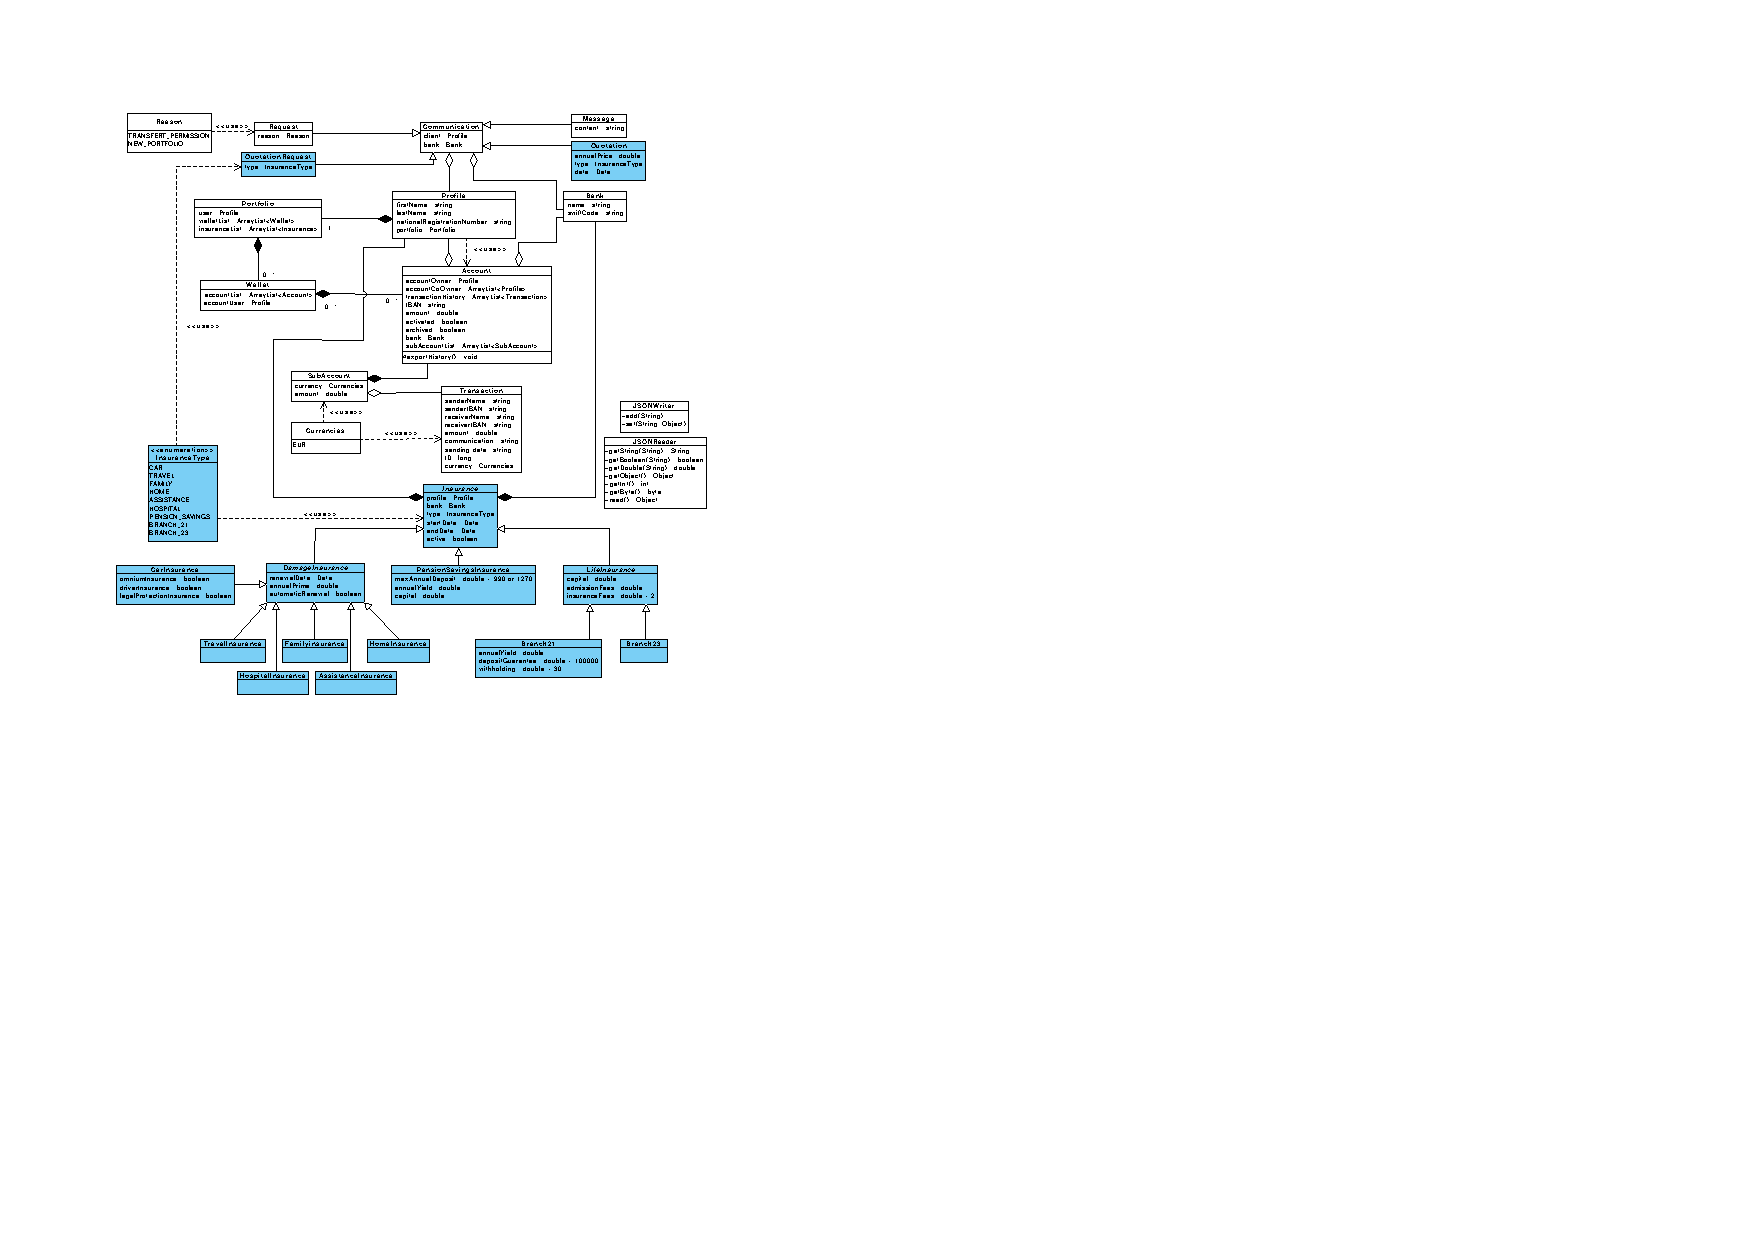
\includegraphics[width=\linewidth]{img/ClassDiagramClientAssurance.pdf}
}
\caption{Diagramme de classe de la partie logique de l'extension assurance}
\end{figure}

\paragraph{Partie logique}La partie logique ne modifie les classes déjà existantes mais en ajoute. Toutes celles-ci sont en commun avec l'application banque. Tout d’abord, on a la classe mère Insurance qui représente une assurance grâce à un assuré et un assureur (Profile et Bank), un type d’assurance, une date de début, une date de fin (Pas forcément définie) et son état d’activité pour savoir si elle est cloturée ou en cours. Chaque type d’assurance possède sa classe fille. Les assurances de dégats sont caractérisées par une date de renouvellement, une prime annuelle et une option pour activer le renouvellement automatique. Seule l’assurance voiture ajoute quelques options supplémentaires à savoir l’assurance omnium, l’assurance conducteur et l’assurance protection juridique. Les assurances épagne pension sont caractérisées par un maximum annuel de dépôt, un rendement annuel et un capital. Les assurances vies sont caractérisées par un capital, des frais d’entrée et des taxes d’assurances. Ces assurances sont sous 2 formes. La première est la branche 21 qui ajoute un rendement annuel, une guarantie de dépôt et un précompte mobilier. La deuxième est la branche 23 et elle n’ajoute rien de plus. Afin de pouvoir gérer les devis entre le client et la banque, deux classes filles de la classe Communication ont été ajoutées. Il s’agit de la classe QuotationRequest qui représente une demande pour un certain type d’assurance et de la classe Quotation qui possède les informations a envoyer au client à savoir la prime anuelle pour un type d’assurance ainsi que la date du devis.

\begin{figure}[ht]
\centering
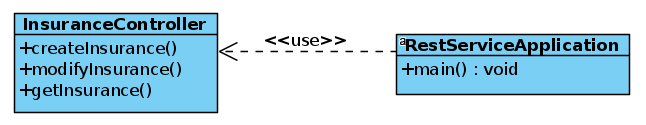
\includegraphics[scale=0.3]{img/APIAssurance.png}
\caption{Ajout au diagramme de classe de la partie de l'extension assurance}
\label{fig2}
\end{figure}

\paragraph{Partie API} La partie API n’ajoute qu’une classe InsuranceController qui permettra de créer, modifier et recevoir une assurance de la base de données. Elle est en commun avec la partie banque.

\begin{figure}[ht]
\centering
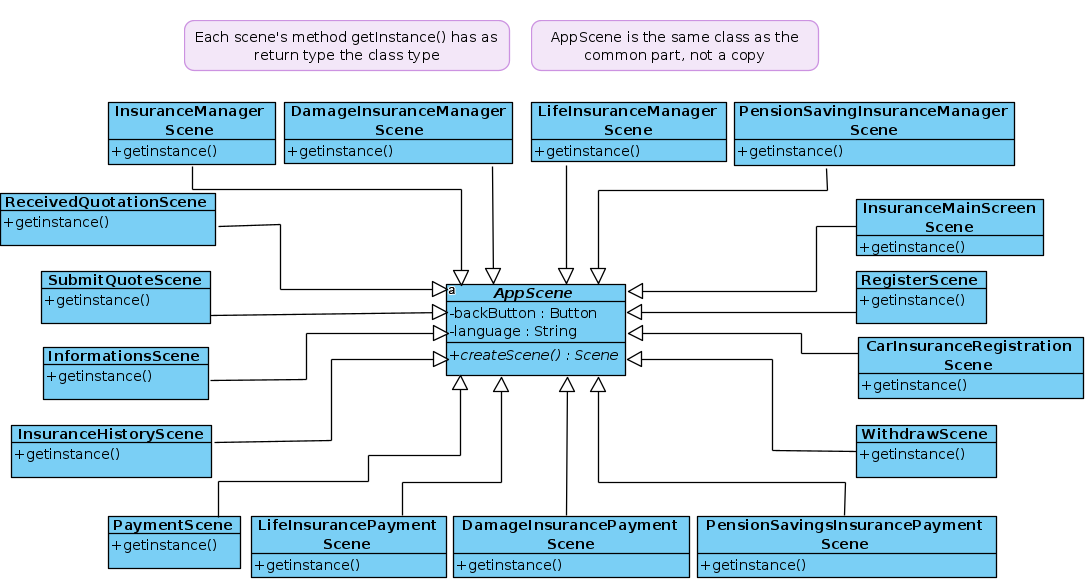
\includegraphics[scale=0.3]{img/GUIAssurance.png}
\caption{Ajout au diagramme de classe de la partie GUI de l'extension assurance}
\label{fig3}
\end{figure}

\paragraph{Partie GUI} La partie GUI ajoute des scenes à la partie de base et ne modifie que le mainScreenScene. Celles-ci héritent tous de AppScene qui est la même classe que la partie commune. Elle a juste isolée du reste de l’application sur le diagramme pour une meilleure visibilité.

\end{document}